\documentclass[a4paper,12pt]{article} 
% 使用ctex包支持中文
\usepackage[UTF8,heading = true]{ctex}
\usepackage[utf8]{inputenc}
\usepackage[T1]{fontenc}
\usepackage{graphicx}
\usepackage{float}
\usepackage{amsmath}
\usepackage{amsfonts}
\usepackage{amssymb}
\usepackage{booktabs}
\usepackage{multirow}
\usepackage{subcaption}
\usepackage{indentfirst}
\usepackage{geometry}
\usepackage{fancyhdr}
\usepackage{ctex}
\usepackage[labelfont=bf]{caption}
\usepackage{listings}
\usepackage{xcolor} % 用于定义自定义颜色和高亮
\usepackage{ragged2e} % 导入ragged2e宏包,用于支持段落两端对齐
\usepackage{cite}

\lstset{
  language=Matlab,              % 设置语言为 MATLAB
  basicstyle=\ttfamily\small,   % 设置基本样式
  keywordstyle=\color{blue},    % 设置关键字样式
  stringstyle=\color{red},      % 设置字符串样式
  commentstyle=\color{green},   % 设置注释样式
  morecomment=[l][\color{magenta}]{\%},   % 对行内注释进行高亮
  morecomment=[s][\color{magenta}]{\%\{}{\%\}},   % 对多行注释进行高亮
  frame=single,                 % 给代码添加框
  rulecolor=\color{black},      % 框的颜色
  numbers=left,                 % 在左侧添加行号
  numberstyle=\tiny\color{gray},% 行号样式
  breaklines=true,              % 自动换行
  postbreak=\mbox{\textcolor{red}{$\hookrightarrow$}\space},
  showstringspaces=false,       % 不特别显示字符串中的空格
  tabsize=2                     % 设置tab为2个空格宽度
}



\geometry{left=3cm,right=3cm,top=3cm,bottom=3cm}

%\ctexset{
    % 修改 section。
    %section={   
        %name={实验,:},
        %number={\chinese{section}},
        %format=\heiti\bfseries\centering\zihao{-2} % 设置 section 标题为黑体、右对齐、小4号字
    %},
    % 修改 subsection。
    %subsection={   
        %name={,、},
        %number={\chinese{subsection}},
        %format=\songti\bfseries\zihao{4} % 设置 subsection 标题为黑体、5号字
    %},
    % 修改 subsection。
    %subsubsection={   
        %name={,、},
        %number={\arabic{subsubsection}},
        %format=\songti\bfseries\zihao{-4} % 设置 subsection 标题为黑体、5号字
    %}
%}
\fancyhead{}


\begin{document}

%制作封面
\begin{titlepage}
    \begin{center}
        \par
            \centerline{
\includegraphics[scale=1.5]{data/media/image1.jpeg} 
\includegraphics[scale=3]{data/media/image2.jpeg}} %插入图片
        \par
		\vskip 5cm
		\lishu \fontsize{50}{20} 实\quad 验\quad 报\quad 告
  
		\vskip 2cm
        \lishu \fontsize{35}{20} 实\quad 验\quad 二
        \vskip 5cm

	\begin{tabular}{l}
		\songti \zihao{-2} \bfseries 课程名称:《数字信号处理实验》
		\quad \\
	    	\songti \zihao{-2} \bfseries 学生姓名:zyh
    
	    	\quad \\
		\songti \zihao{-2} \bfseries 学生学号:202264691103
		\quad \\
	    	\songti \zihao{-2} \bfseries 学生专业:人工智能
	    	\quad \\
	     \songti \zihao{-2} \bfseries 开课学期:2023-2024年第二学期
	     \quad \\
           \songti \zihao{-2} \bfseries  提交日期:2024年5月8日
    \end{tabular}
    \end{center}
\end{titlepage}


% 生成目录
\newpage
\pagestyle{empty}
\begin{center}
\tableofcontents
\end{center}

\newpage

\setcounter{page}{1}

\section{验证性实验}
\subsection{实验目的}
\begin{itemize}
    \item 研究和验证不同频率成分的信号叠加及其频谱特性
    \item 验证指数序列的离散傅里叶变换(DFT)和其逆变换(IDFT)的效果
    \item 验证离散傅里叶变换(DFT)的对称性和共轭对称性
\cite{ning2012}
    
\end{itemize}


\subsection{实验原理}
\subsubsection{信号的频率分解}
信号 \( x[n] \) 可以表示为不同频率正弦波的叠加:
\begin{equation}
x[n] = \sum_{k=0}^{N-1} A_k \cos(2\pi f_k nT + \phi_k) 
\end{equation}

其中,\( A_k \),\( f_k \),和 \( \phi_k \) 分别是第 \( k \) 个正弦波的幅度、频率和相位,\( T \) 是采样周期,\( n \) 是时域的采样点索引。

\subsubsection{离散傅里叶变换(DFT)}
离散傅里叶变换提供了一种方法,可以将时域的离散信号转换为频域的表示。DFT定义为:
\begin{equation}
X[k] = \sum_{n=0}^{N-1} x[n] \cdot e^{-j\frac{2\pi}{N}kn}
\end{equation}

其中,\( X[k] \) 是在频率索引 \( k \) 处的复数形式的频域表示,展示了频率 \( \frac{k}{NT} \) 处的幅度和相位信息。

对于基本的指数序列,其DFT可以直接计算为:
\begin{equation}
X[k] = \sum_{n=0}^{N-1} x[n] \cdot e^{-j\frac{2\pi}{N}kn}
\end{equation}

这一公式揭示了序列在离散频率点 \( k \) 的复振幅,其中包含了幅度和相位信息。对于纯指数信号,DFT结果在特定 \( k \) 值处会显示为尖峰,此 \( k \) 值对应于指数序列的频率 \( \omega_0 \)。

\subsubsection{频谱分析和频率成分的可视化}

通过计算 \( X[k] \) 的幅度和相位,我们可以获得信号的频谱图。幅度谱 \( |X[k]| \) 和相位谱 \( \angle X[k] \) 分别提供了不同频率成分的强度和相位偏移信息:
\begin{equation}
|X[k]| = \sqrt{\text{Re}(X[k])^2 + \text{Im}(X[k])^2}
\end{equation}

\begin{equation}
\angle X[k] = \arctan\left(\frac{\text{Im}(X[k])}{\text{Re}(X[k])}\right)
\end{equation}


\subsubsection{信号重构}

利用逆离散傅里叶变换(IDFT),可以从频域数据 \( X[k] \) 重构原始时域信号 \( x[n] \):
\begin{equation}
x[n] = \frac{1}{N} \sum_{k=0}^{N-1} X[k] \cdot e^{j\frac{2\pi}{N}kn}
\end{equation}

这一过程表明,通过适当处理其频域表示,原始信号可以完整地恢复,证明了频率成分分析的准确性和有效性。

\subsubsection{IDFT的应用}
逆离散傅里叶变换(IDFT)是DFT的逆过程,用于从频域信号恢复时域信号:
\begin{equation}
x[n] = \frac{1}{N} \sum_{k=0}^{N-1} X[k] \cdot e^{j\frac{2\pi}{N}kn}
\end{equation}
通过IDFT,可以验证DFT的准确性。如果从DFT到IDFT的转换能完美地重构原始信号 \( x[n] \),则证明了变换过程的正确性和信号处理方法的有效性。

\subsubsection{指数序列和其变换}

指数序列一般形式为 \( x[n] = A e^{j(\omega_0 n + \phi)} \),其中 \( A \)、\( \omega_0 \) 和 \( \phi \) 分别代表幅度、基本角频率和相位。此类序列在进行离散傅里叶变换时,显示为频谱中的尖峰,这一特性使其在频域分析中尤为重要。

\subsubsection{离散傅里叶变换(DFT)的对称性和共轭对称性}
\begin{itemize}
    \item 对称性

    在DFT中,如果输入信号是实数(即 \( x[n] \) 没有虚部),那么其频谱将展示对称性。具体来说,对于 \( N \) 点DFT,有:
\[ X[k] = X[N-k]^* \]
这意味着频谱的第 \( k \) 项和第 \( N-k \) 项是共轭对称的,即它们的幅度相等,相位相反。

    \item 共轭对称性

如果输入信号是纯实数的偶函数(即 \( x[n] = x[N-n] \)),其DFT结果也将是实数且偶对称。类似地,如果输入信号是纯实数的奇函数(即 \( x[n] = -x[N-n] \)),其DFT结果将是纯虚数且奇对称。

    \item 数学描述和公式
    
对于一个一般的复数信号,DFT定义为:
\begin{equation}
X[k] = \sum_{n=0}^{N-1} x[n] \cdot e^{-j\frac{2\pi}{N}kn}
\end{equation}

通过这一定义,我们可以展开并验证信号的共轭对称性。对于实数信号,我们有:
\begin{equation}
X[k] = \sum_{n=0}^{N-1} x[n] \cdot \cos\left(\frac{2\pi kn}{N}\right) - j\sum_{n=0}^{N-1} x[n] \cdot \sin\left(\frac{2\pi kn}{N}\right)
\end{equation}

其中实部和虚部的对称性可以独立检验。
    
\end{itemize}

通过验证DFT的对称性和共轭对称性,不仅加强了对信号频谱结构的理解,还为信号分析提供了重要的数学工具。这些性质在减少计算量、提高算法效率以及实际信号处理系统的设计中发挥着关键作用,尤其是在音频和通信领域中。

\subsection{实验内容}
\begin{itemize}
    \item 1. 2N点实数序列
\[
x(n) = 
\begin{cases} 
\cos\left(\frac{2\pi \cdot 7n}{N}\right) + \frac{1}{2} \cos\left(\frac{2\pi \cdot 19n}{N}\right), & n = 0,1,2,\ldots,2N-1; \\
0, & \text{其他} n;
\end{cases}
\]
N=64。用一个64点的复数FFT 程序,一次算出,$X(k) = \text{DFT}[x(n)]_{2N}$并绘出$|X(k)|$的图形。

    \item 2. 已知指数序列在单位圆上的 $N=64$ 点分布的 $Z$ 变换为:
\[
X(Z_k) = X(k) = \frac{1}{1 - 0.8e^{-j2\pi k/N}}, \quad k = 0,1,2,\ldots,63
\]
用 $N$ 点 IFFT 程序计算出 $\bar{x}(n) = \text{IDFT}[X(k)]$ 和 $\bar{x}(n)$。

    \item 3. 使用Matlab编程验证DFT操作的对称性。设计您自己的N点复序列,并通过编程验证表5.1中的对称性属性。
    
    \centering 
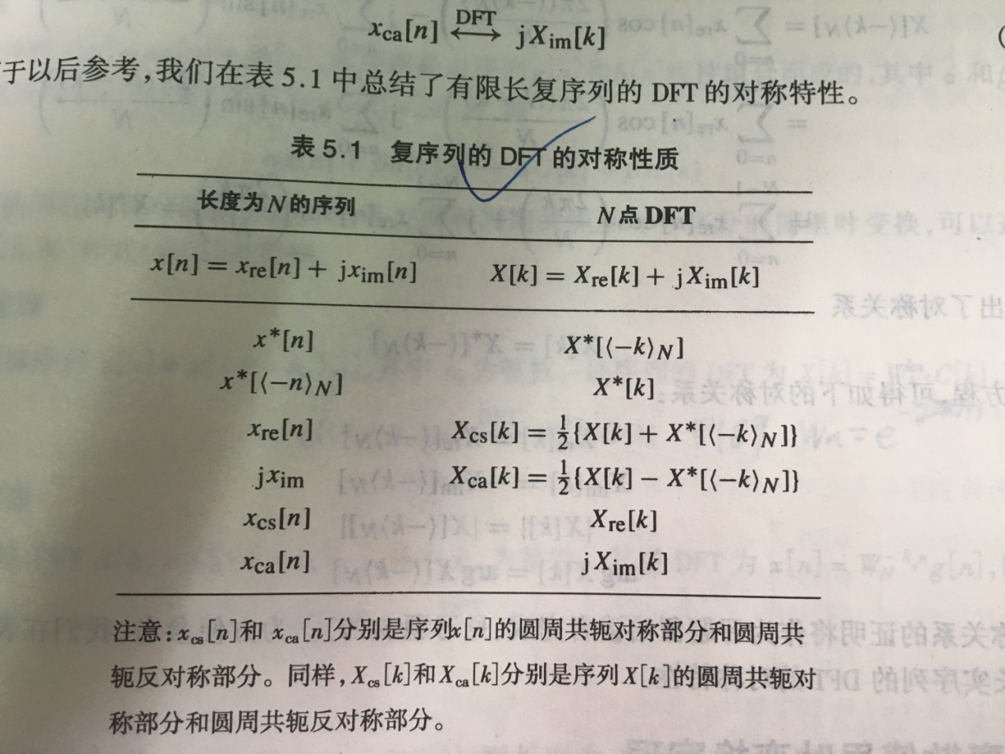
\includegraphics[width=0.8\linewidth]{images/2_Verify/Question.png}
\captionof{figure}{实验要求} 
\justifying

\end{itemize}

\subsubsection{实验一}
\begin{itemize}
\item 首先,定义了一个序列的长度 $N$ 为 64,然后创建了一个时间索引 $n$,范围从 0 到 $2N-1$。
\item 接下来,定义了一个信号 $x$,它是两个正弦信号的叠加,分别以不同的频率振荡。第一个正弦信号的频率为 7 Hz,第二个正弦信号的频率为 19 Hz。
\item 使用快速傅里叶变换(FFT)计算了信号 $x$ 的频谱,得到了频谱 $X$。
\item 计算了频谱的幅度 $|X(k)|$,即频谱的绝对值。
\item 最后,绘制了频谱幅度 $|X(k)|$ 的图形,使用了 \texttt{stem} 函数来绘制离散点图。横坐标表示频率索引 $k$,纵坐标表示幅度,同时添加了标签和标题以及网格线。
\end{itemize}

\begin{lstlisting}
N = 64; % 序列长度
n = 0:2*N-1; % 时间索引 n

% 定义信号 x(n)
x = cos(2*pi*7*n/N) + 1/2*cos(2*pi*19*n/N);

% 计算信号的快速傅里叶变换(FFT)
X = fft(x, 2*N);

% 计算幅度 |X(k)|
magnitude_X = abs(X);

% 绘制 |X(k)| 的图形
k = 0:2*N-1; % 频率索引 k
stem(k, magnitude_X); % 使用 stem 函数来绘制离散点
xlabel('k');
ylabel('|X(k)|');
title('Magnitude of DFT of x(n)');
grid on;

\end{lstlisting}

可以得到以下实验结果:
    
\centering 
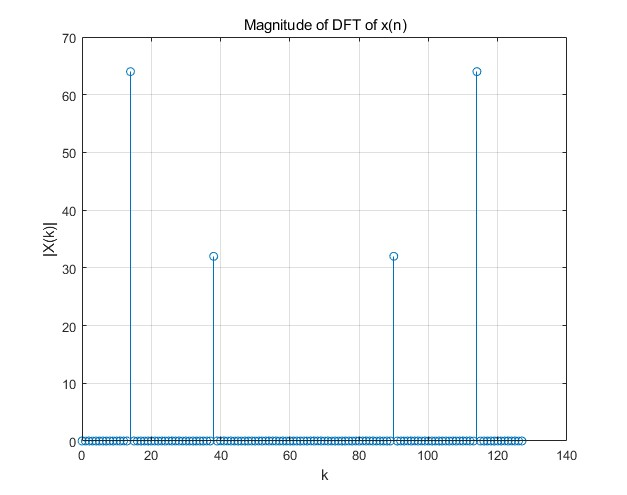
\includegraphics[width=0.8\linewidth]{images/2_Verify/verify1.jpg}
\captionof{figure}{不同频率成分的信号叠加及其频谱特性} 
\justifying

\subsubsection{实验二}
\begin{itemize}
    \item 定义了一个序列的点数为 \( N = 64 \),并创建了一个点的索引 \( k \),范围从 0 到 \( N-1 \)。
    \item 计算了序列 \( X(k) \) 在单位圆上的 64 个点。这里使用了一个公式来计算 \( X(k) \),公式为 \( X(k) = \frac{1}{1 - 0.8 \cdot e^{-j2\pi k/N}} \),其中 \( j \) 是虚数单位。
    \item 通过使用逆离散傅里叶变换(IFFT),计算了序列 \( x(n) \)。在 MATLAB 中,可以使用 \texttt{ifft} 函数来执行逆离散傅里叶变换。
    \item 由于原始序列是复数,但实际应用中通常处理实数序列,因此将计算得到的序列取了实部。
    \item 显示了计算得到的序列 \( x(n) \)。
    \item 使用了 \texttt{stem} 函数绘制了序列 \( x(n) \) 的图形,横坐标表示序列索引 \( n \),纵坐标表示序列值 \( x(n) \),并添加了标签和标题。
\end{itemize}

\begin{lstlisting}
N = 64; % 序列的点数
k = 0:N-1; % 点的索引

% 计算序列X(k)在单位圆上的64点
X_k = 1 ./ (1 - 0.8 .* exp(-1j * 2 * pi * k / N));

% 计算x(n)通过使用IFFT
x_n = ifft(X_k);

% 因为原始序列是实数,取实部
x_n = real(x_n);

% 显示序列
disp(x_n);

% 可视化序列
stem(0:N-1, x_n);
xlabel('n');
ylabel('x(n)');
title('Sequence x(n) from IFFT');

\end{lstlisting}

可以得到以下的实验结果:
\centering 
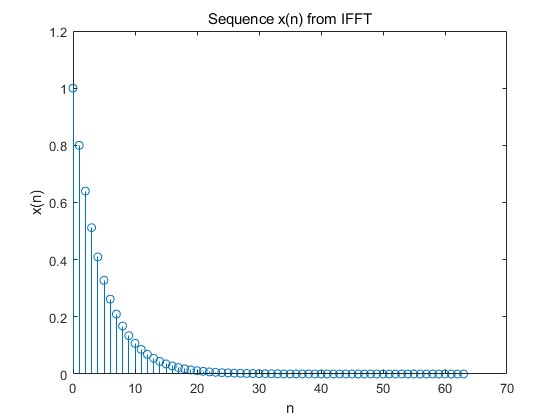
\includegraphics[width=0.8\linewidth]{images/2_Verify/verify2.jpg}
\captionof{figure}{} 
\justifying

\subsubsection{实验三}
以下代码实现了对给定复数序列的各种对称性分析,并对其进行了离散傅里叶变换(DFT),然后绘制了不同情况下的DFT结果。

下面是关于这段代码的说明:

\begin{itemize}
    \item 定义了一个包含复数元素的序列 \( x \),这个序列有四个元素。
    \item 计算了序列的长度 \( N \),并创建了一个序列的索引 \( n \),范围从 0 到 \( N-1 \)。
    \item 分别提取了序列 \( x \) 的实部、虚部和共轭部分,并构造了 \( x \) 的倒序序列 \( xr \) 和其共轭序列 \( x_cc \)。
    \item 计算了序列 \( x \) 的共轭序列 \( x_cc \) 和 \( x \) 的共轭序列 \( x_cc \) 在频域的DFT。
    \item 计算了 \( x \) 的实部序列 \( x_re \) 和 \( x \) 的虚部序列 \( x_im \) 在频域的DFT。
    \item 计算了 \( x \) 的共轭序列 \( x_cc \) 和 \( x \) 的平均序列 \( x_cs \) 在频域的DFT。
    \item 计算了 \( x \) 的共轭序列 \( x_cc \) 和 \( x \) 的差分序列 \( x_ca \) 在频域的DFT。
    \item 使用 \texttt{stem} 函数绘制了不同情况下的DFT结果的实部和虚部,分别包括 \( x \) 的共轭序列、实部、虚部、共轭序列的DFT结果,以及共轭序列和实部序列的平均、差分序列的DFT结果。
    \item 每个图形都包括了四个子图,分别展示了实部和虚部的DFT结果。
\end{itemize}

\begin{lstlisting}
function varargout=symmetry()
x=[1+1j*4, -1+1j*3, 4-1j*2, -5-1j*6];
N=length(x);
n=0:N-1;
x_re=real(x);
x_im=imag(x);
x_conj=conj(x);
xr=x(mod(-n,N)+1);
x_cc=conj(xr);
% x_cc=[1-1j*4, -5+1j*6, 4+1j*2, -2-1j*3];
% x_cs=[1, -3.5+1j*4.5, 4, -3.5-1j*4.5];
% x_ca=[1j*4, 1.5-1j*1.5,-1j*2,-1.5-1j*1.5];
x_cs=0.5*(x+x_cc);
x_ca=0.5*(x-x_cc);

k=0:N-1;
Xk=fft(x);
Xkr=Xk(mod(-k,N)+1);
Xk_cc=conj(Xkr);
Xk_conj=conj(Xk);
Xk_re=real(Xk);
Xk_im=imag(Xk);
Xk_cs=0.5*(Xk+Xk_cc);
Xk_ca=0.5*(Xk-Xk_cc);

X1=fft(x_conj);
X2=fft(x_cc);
X3=fft(x_re);
X4=fft(1j.*x_im);
X5=fft(x_cs);
X6=fft(x_ca);

figure
subplot(2,2,1)
stem(k,real(X1))
title('real part of DFT[x*[n]]')
subplot(2,2,2)
stem(k,imag(X1))
title('imag part of DFT[x*[n]]')
subplot(2,2,3)
stem(k,real(Xk_cc))
title('real part of X*[<-k>N]')
subplot(2,2,4)
stem(k,imag(Xk_cc))
title('imag part of X*[<-k>N]')

figure
subplot(2,2,1)
stem(k,real(X2))
title('real part of DFT[x*[<-n>N]]')
subplot(2,2,2)
stem(k,imag(X2))
title('imag part of DFT[x*[<-n>N]]')
subplot(2,2,3)
stem(k,real(Xk_conj))
title('real part of X*[k]')
subplot(2,2,4)
stem(k,imag(Xk_conj))
title('imag part of X*[k]')

figure
subplot(2,2,1)
stem(k,real(X3))
title('real part of DFT[xre[n]]')
subplot(2,2,2)
stem(k,imag(X3))
title('imag part of DFT[xre[n]]')
subplot(2,2,3)
stem(k,real(Xk_cs))
title('real part of Xcs[k]')
subplot(2,2,4)
stem(k,imag(Xk_cs))
title('imag part of Xcs[k]')

figure
subplot(2,2,1)
stem(k,real(X4))
title('real part of DFT[jxim[n]]')
subplot(2,2,2)
stem(k,imag(X4))
title('imag part of DFT[jxim[n]]')
subplot(2,2,3)
stem(k,real(Xk_ca))
title('real part of Xca[k]')
subplot(2,2,4)
stem(k,imag(Xk_ca))
title('imag part of Xca[k]')

figure
subplot(2,2,1)
stem(k,real(X5))
title('real part of DFT[xcs[n]]')
subplot(2,2,2)
stem(k,imag(X5))
title('imag part of DFT[xcs[n]]')
subplot(2,2,3)
stem(k,real(Xk_re))
title('real part of Xre[k]')
subplot(2,2,4)
stem(k,imag(Xk_re))
title('imag part of Xre[k]')

figure
subplot(2,2,1)
stem(k,real(X6))
title('real part of DFT[xca[n]]')
subplot(2,2,2)
stem(k,imag(X6))
title('imag part of DFT[xca[n]]')
subplot(2,2,3)
stem(k,real(1j*Xk_im))
title('real part of jXim[k]')
subplot(2,2,4)
stem(k,imag(1j*Xk_im))
title('imag part of jXim[k]')
\end{lstlisting}

得到的结果如下:
\begin{figure}[h]
    \centering
    \begin{minipage}[b]{0.48\textwidth}
        \centering
        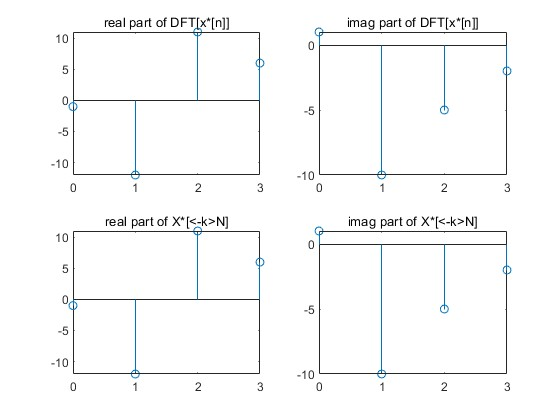
\includegraphics[width=\linewidth]{images/2_Verify/symmetry1.jpg}
        \caption{对称性分析1}
    \end{minipage}
    \hfill
    \begin{minipage}[b]{0.48\textwidth}
        \centering
        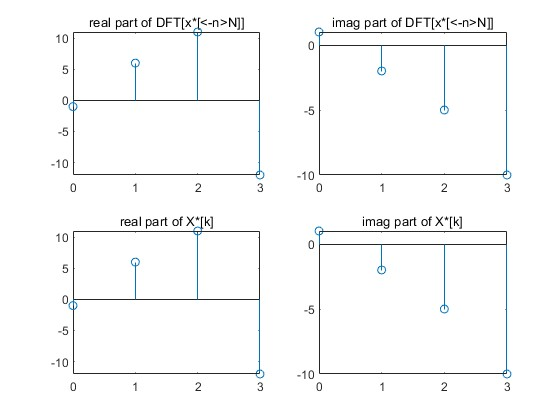
\includegraphics[width=\linewidth]{images/2_Verify/symmetry2.jpg}
        \caption{对称性分析2}
    \end{minipage}
\end{figure}

\begin{figure}[h]
    \centering
    \begin{minipage}[b]{0.48\textwidth}
        \centering
        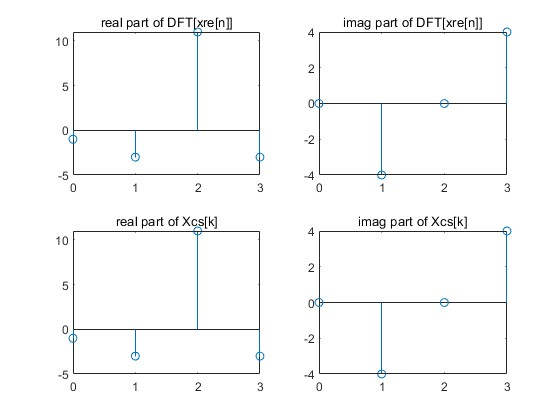
\includegraphics[width=\linewidth]{images/2_Verify/symmetry3.jpg}
        \caption{对称性分析3}
    \end{minipage}
    \hfill
    \begin{minipage}[b]{0.48\textwidth}
        \centering
        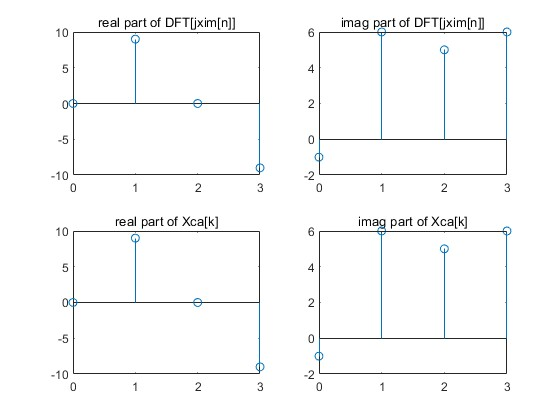
\includegraphics[width=\linewidth]{images/2_Verify/symmetry4.jpg}
        \caption{对称性分析4}
    \end{minipage}
\end{figure}

\begin{figure}[h]
    \centering
    \begin{minipage}[b]{0.48\textwidth}
        \centering
        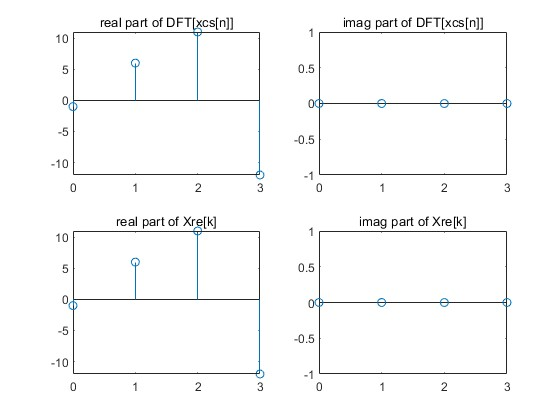
\includegraphics[width=\linewidth]{images/2_Verify/symmetry5.jpg}
        \caption{正弦序列、复指数序列性质3}
    \end{minipage}
    \hfill
    \begin{minipage}[b]{0.48\textwidth}
        \centering
        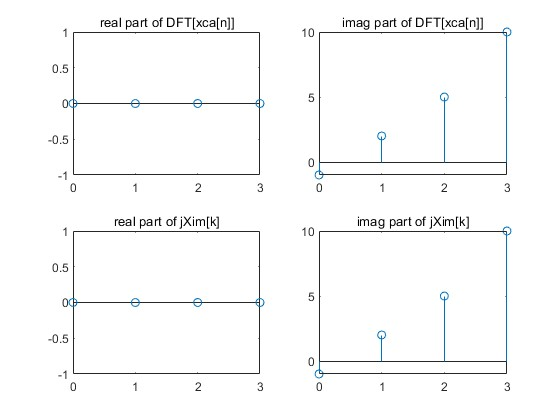
\includegraphics[width=\linewidth]{images/2_Verify/symmetry6.jpg}
        \caption{正弦序列、复指数序列性质4}
    \end{minipage}
\end{figure}


\newpage

\section{应用性实验}
\subsection{实验目的}
使用至少两种频率估计方法对给定信号进行频率估计。

\subsection{实验原理}
\subsubsection{频率估计方法的选择与原理}
\begin{itemize}
    \item 频率估计方法的分类:频率估计方法主要分为时域方法和频域方法两大类。时域方法通常基于信号周期性特征,如自相关函数、互相关函数等,而频域方法则基于信号的频谱特征,如周期图、功率谱密度等。
    \item 经典频率估计方法:经典频率估计方法包括周期图法、自相关法、最小均方误差法、Yule-Walker法等。这些方法在信号处理领域有着广泛的应用,并且具有一定的数学理论基础。
    \item 基于傅里叶变换的频率估计方法:基于傅里叶变换的频率估计方法利用傅里叶变换将时域信号转换到频域,通过分析频域特征来估计信号的频率。常见的方法包括周期图法、平均幅度差谱法、高分辨率频谱估计法等。
    \item 选择适合实际应用的方法:不同的频率估计方法适用于不同的信号特性和实际应用场景。在选择频率估计方法时,需要考虑信号的特性、噪声水平、计算复杂度等因素,并根据具体情况选取最合适的方法。
    \item 评估频率估计结果的准确性:对于每种频率估计方法,都需要评估其对信号频率的估计准确性。通常使用均方误差或者其他指标来衡量估计结果与真实值之间的差距,以便对不同方法进行比较和分析。
\end{itemize}

\subsubsection{FFT基本原理及其在频率估计中的应用。}
FFT(快速傅里叶变换)是一种高效的计算傅里叶变换的算法,它将离散傅里叶变换(DFT)的计算复杂度从 \(O(N^2)\) 降低到了 \(O(N \log N)\),其中 \(N\) 是信号的长度。其基本原理是通过分治策略,将长度为 \(N\) 的序列分解成长度为 \(N/2\) 的子序列,并利用旋转因子的性质将其逐步合并,最终得到完整的频域表示。

在频率估计中,FFT广泛应用于计算信号的频谱。其基本思想是将信号转换到频域,在频域中对信号进行分析和处理。通过计算信号的FFT,可以得到信号在频率域上的表示,从而实现频率估计。

FFT在频率估计中的应用主要体现在以下几个方面:
\begin{itemize}
    \item \textbf{频谱分析:} FFT可以将信号从时域转换到频域,得到信号的频谱。频谱分析可以用于确定信号中的频率成分及其强度,从而进行频率估计。
    \item \textbf{谱线提取:} 通过对FFT结果进行峰值检测或频谱分析,可以提取信号中的主要频率成分,从而进行频率估计。
    \item \textbf{相关性分析:} FFT可以用于计算信号之间的相关性,进而可以在频域上对信号进行相关性分析,从而进行频率估计。
\end{itemize}

在实际应用中,FFT通常与其他频率估计方法结合使用,例如基于周期图法或最小均方误差法的频率估计方法,以提高估计精度和准确性。

\subsubsection{信噪比的概念与计算方法}
信号功率 $P_s$ 的计算公式为: 
\[ P_s = \frac{1}{N} \sum_{n=0}^{N-1} |x(n)|^2 \]

其中,$N$ 是信号的样本点数,$x(n)$ 是信号在时域上的离散样本值。
\begin{itemize}
    \item \textbf{噪声功率的计算:} 类似地,对于给定的噪声信号,可以通过计算噪声的功率来评估其强度。噪声的功率通常通过信号中的噪声样本值的平方的均值来计算。

    噪声功率 $P_n$ 的计算公式为: 
\[ P_n = \frac{1}{N} \sum_{n=0}^{N-1} |e(n)|^2 \]

其中,$e(n)$ 是信号中的噪声样本值。

    \item \textbf{信噪比的计算:} 信噪比是信号功率与噪声功率之比,通常以分贝为单位表示。信噪比的计算公式为:
    \begin{equation}
        SNR_{\text{dB}} = 10 \log_{10} \left( \frac{P_s}{P_n} \right)
    \end{equation}

其中,$SNR_{\text{dB}}$ 是以分贝表示的信噪比,$P_s$ 是信号功率,$P_n$ 是噪声功率。
\end{itemize}



\subsubsection{AWGN的生成与信号加噪处理}
\begin{itemize}
    \item \textbf{AWGN的生成:} AWGN是一种常见的噪声模型,通常用于模拟真实环境中的噪声情况。它具有高斯分布和白噪声特性,即在频率上具有均匀分布的功率谱密度。在数字信号处理中,可以使用随机数生成方法来产生AWGN。
    
    \item \textbf{AWGN的特性:} AWGN的特点包括均值为0、方差为$\sigma^2$,其中$\sigma^2$表示噪声的功率。在信号加噪处理中,可以将AWGN加到原始信号中,以模拟信号在噪声环境中的表现。
    
    \item \textbf{信号加噪处理:} 在信号处理中,通常会将AWGN加到原始信号中,以模拟信号在真实环境中的传输过程。信号加噪处理的过程可以通过将AWGN的样本值加到原始信号的样本值上来实现。加噪后的信号可以用于评估信号处理算法在噪声环境中的性能。
\end{itemize}

通过生成AWGN并将其加到原始信号中,可以模拟在不同信噪比下的信号场景,进而进行信号处理算法的性能评估。

\subsection{实验内容}
\subsubsection{Rife算法实现频率估计}
Rife算法(也称为Rife-Zhilin算法)是一种常用于频率估计的信号处理算法,特别适用于单频或多频信号的频率估计。该算法基于峰值检测和迭代优化的思想,能够有效地估计信号的频率成分。\cite{rife1989digital}

以下是Rife算法的主要步骤和原理:
\begin{itemize}
    \item \textbf{信号预处理:} 首先,对原始信号进行预处理,通常包括去趋势、滤波等操作,以减少噪声的影响,并提高频率估计的准确性。
    
    \item \textbf{峰值检测:} 利用峰值检测方法(如寻找局部最大值)找到FFT(快速傅里叶变换)结果中的峰值,这些峰值对应于信号的频率成分。
    
    \item \textbf{初始化参数:} 根据峰值检测结果,初始化估计的频率参数,如初始频率值和步长等。
    
    \item \textbf{迭代优化:} 使用迭代优化方法(如最小二乘法或牛顿法),不断调整频率参数,使得信号模型在时域和频域上与原始信号的拟合度最大化。
    
    \item \textbf{收敛判断:} 在迭代过程中,通过设置收敛条件(如迭代次数或残差阈值),判断算法是否收敛,如果满足收敛条件,则停止迭代,否则继续迭代调整参数。
    
    \item \textbf{频率估计:} 最终得到收敛后的频率参数作为对信号频率成分的估计结果。
\end{itemize}

根据描述,可以得到以下思路:

\begin{itemize}
    \item \textbf{输入参数}:
    \begin{itemize}
        \item \texttt{spec}:信号频谱列向量或以列向量叠加的矩阵。
        \item \texttt{fs}:信号的采样率。
    \end{itemize}
    
    \item \textbf{输出参数}:
    \begin{itemize}
        \item \texttt{fc}:Rife 算法估计出的频率。
    \end{itemize}
    
    \item \textbf{主要步骤}:
    \begin{enumerate}
        \item 计算信号频谱中的峰值和对应的位置。
        \item 根据峰值的位置以及频谱的形状,利用 Rife 算法估计出信号的频率。
        \item 将估计得到的频率存储在输出向量 \texttt{fc} 中。
    \end{enumerate}
    
    \item \textbf{代码逻辑}:
    \begin{enumerate}
        \item 通过 \texttt{max} 函数找到频谱中的峰值及其位置。
        \item 对每个峰值位置进行处理,根据 Rife 算法的公式估计频率。
        \item 最终得到的频率存储在输出向量 \texttt{fc} 中,并返回给调用函数。
    \end{enumerate}
\end{itemize}

\begin{lstlisting}
function fc = rife_function(spec,fs)
%Rife算法matlab实现
%   spec:信号频谱列向量或以列向量叠加的矩阵
%   fs:信号采样率
%   输出fc为Rife算法估计出的频率
[length,SignalNum] = size(spec);
[valueMax,posMax] = max(spec(length/2+1:length,:));
disp(posMax)
T = length/fs;
for k = 1:SignalNum
    r= 2*((spec(posMax(k)+length/2,k) > spec(posMax(k)+length/2-2,k))-0.5);
    rat =spec(posMax(k)+length/2+r-1,k) /(valueMax(k)+spec(posMax(k)+length/2+r-1,k));
    % rat = valueMax(k)/(valueMax(k)+spec(posMax(k)+length/2+r-1,k));
    fc(k) = 1/T*(posMax(k)+r*rat-2);
end
end

\end{lstlisting}

得到的结果如下:

\centering 
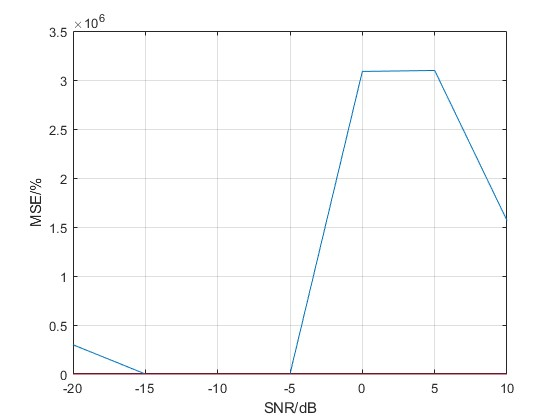
\includegraphics[width=0.8\linewidth]{images/2_Application/Rife.jpg}
\captionof{figure}{Rife算法频率估计结果} 
\justifying

图中显示了信号的均方误差(MSE)随信噪比(SNR)的变化情况。从图中可以看出,随着SNR从5dB逐渐增加到10dB,MSE显著地降低,这意味着信号的估计误差减少,频率估计的精确度提高。当SNR达到-5dB左右时,MSE达到最小,这表明这个SNR水平下Rife算法能够非常准确地估计出频率。然而,当SNR继续增加至0dB和5dB时,MSE突然增大,表明在这些较高的信噪比下,Rife算法的性能反而下降,可能是由于过拟合或其他数值计算问题导致的。

这种MSE在高SNR值时上升的情况可能是由算法在处理过于清晰的信号时引入的额外误差,或者是FFT计算中的一些特定的数值问题,如频谱泄漏或窗函数的影响。这个结果提示在实际应用中,当信噪比较高时,可能需要对Rife算法进行调整或优化,以保持频率估计的准确性。


\subsubsection{Pisarenko 谐波分解算法实现频率估计}

\begin{itemize}
    \item \textbf{基本原理:} Pisarenko 谐波分解算法基于信号的自相关矩阵来进行频率估计。该算法假设信号是由正弦波成分构成的,并且在给定的噪声条件下,可以通过分解自相关矩阵来估计信号的频率。\cite{pisarenko1973retrieval}
    
    \item \textbf{算法步骤:}
    \begin{enumerate}
        \item 构建自相关矩阵:对于给定的信号,首先计算其自相关矩阵。
        \item 特征值分解:对自相关矩阵进行特征值分解,得到特征值和对应的特征向量。
        \item 频率估计:通过特征值和特征向量,可以估计信号中的频率成分。通常情况下,特征值中最小的非零特征值对应的特征向量中包含了信号的频率信息,通过对应的特征向量可以估计出频率。
    \end{enumerate}
    
    \item \textbf{优缺点:}
    \begin{itemize}
        \item 优点:Pisarenko 谐波分解算法具有较好的频率分辨率和估计精度,在一定条件下对于单频信号有较好的估计效果。
        \item 缺点:该算法对于多频信号的处理效果较差,且在存在噪声干扰较大时容易受到影响。
    \end{itemize}
    
    \item \textbf{应用领域:} Pisarenko 谐波分解算法常被应用于信号处理、通信系统、雷达系统等领域,用于提取信号中的频率成分,进行频率估计和谱分析。
\end{itemize}

根据描述,可以得到以下思路:

\begin{itemize}
    \item 初始化输出频率数组 \texttt{fc}。
    \item 对于每个输入信号,执行以下步骤:
    \begin{itemize}
        \item 获取单列频谱数据 \texttt{spectrum}。
        \item 计算频谱的自相关。
        \item 使用自相关值构建 Toeplitz 矩阵 \texttt{R}。
        \item 对 \texttt{R} 进行特征分解,得到特征向量和特征值。
        \item 找到具有最小特征值的特征向量,这个特征向量对应着信号中的主要频率成分。
        \item 通过特征向量计算频率估计值 \texttt{phd\_freq}。
        \item 修正频率估计,确保其为正值(因为 \texttt{atan2} 的范围是 $-\pi$ 到 $\pi$)。
        \item 存储计算得到的频率估计值到输出数组 \texttt{fc} 中。
    \end{itemize}
\end{itemize}

\begin{lstlisting}
function fc = phd_function(spec, fs)
    %Pisarenko谐波分解算法的MATLAB实现
    %   spec: 信号频谱列向量或以列向量叠加的矩阵
    %   fs: 信号采样率
    %   输出fc为Pisarenko算法估计出的频率

    % 获取信号的大小信息
    [nfft, signalNum] = size(spec);
    fc = zeros(1, signalNum); % 初始化输出频率数组
    
    % 对每个信号进行处理
    for k = 1:signalNum
        % 获取单列频谱数据
        spectrum = spec(:, k);

        % 计算自相关
        autocorr_values = ifft(abs(spectrum).^2);

        % 生成自相关矩阵
        R = toeplitz(autocorr_values(1:nfft/2+1));

        % 特征分解
        [eigenvectors, eigenvalues] = eig(R);
        
        % 找到最小的特征值对应的特征向量
        [min_eigenvalue, min_index] = min(abs(diag(eigenvalues)));
        phd_vector = eigenvectors(:, min_index);
        
        % 计算频率,假设为单频信号
        phd_freq = fs / (2 * pi) * atan2(imag(phd_vector(2)), real(phd_vector(1)));
        
        % 修正频率估计,保证其为正值
        if phd_freq < 0
            phd_freq = phd_freq + fs/2;
        end
        
        % 存储计算的频率
        fc(k) = phd_freq;
    end
end

\end{lstlisting}

可以得到以下结果:
\centering 
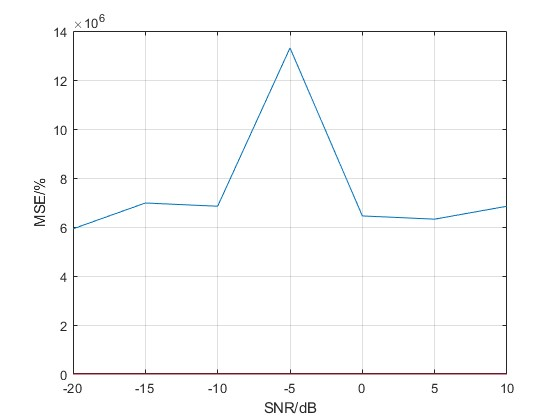
\includegraphics[width=0.8\linewidth]{images/2_Application/phd.jpg}
\captionof{figure}{Pisarenko 谐波分解算法频率估计结果} 
\justifying

这张图展示了使用Pisarenko谐波分解算法进行频率估计时,均方误差(MSE)随信噪比(SNR)变化的情况。与前面的Rife算法相比,Pisarenko算法在某些SNR值上表现出更高的误差。

从图中可以观察到,在SNR达到-5dB附近时,MSE急剧上升到一个峰值,表明在这一点上,算法的性能显著恶化。之后,当SNR继续增加至0dB和10dB,MSE又逐渐降低。

这种在特定SNR值(-5dB)附近性能恶化的现象可能与Pisarenko算法在处理接近平衡信噪比条件时的内部数值不稳定性有关。这表明虽然Pisarenko算法在低噪声或高噪声的环境下能够较好地估计频率,但在某些特定的信噪比水平下可能需要额外的稳定化措施或参数调整来提高其鲁棒性。

\subsubsection{MUSIC算法实现频率估计}
MUSIC(Multiple Signal Classification)算法是一种用于频率估计的经典算法,特别适用于估计具有稀疏频率成分的信号的频率。该算法最初由Schmidt于1986年提出,主要用于信号处理和谱估计。\cite{schmidt1986multiple}

以下是MUSIC算法的基本原理:
\begin{itemize}
    \item \textbf{构建数据矩阵:} 首先,将接收到的信号数据转换为数据矩阵形式,其中每一列表示一个接收到的信号样本.
    
    \item \textbf{计算信号空间协方差矩阵:} 对数据矩阵进行协方差矩阵的计算,该矩阵反映了信号的统计特性.
    
    \item \textbf{特征分解:} 对信号空间协方差矩阵进行特征分解,得到特征向量和特征值.
    
    \item \textbf{构建伪谱密度函数:} 利用特征向量构建伪谱密度函数(Pseudo Spectrum),这是MUSIC算法的核心. 该函数用于估计信号的频率成分.
    
    \item \textbf{频率估计:} 通过分析伪谱密度函数,识别出峰值对应的频率作为信号的频率估计值.
\end{itemize}


MUSIC算法的优点之一是对信号中存在的多个频率成分具有较好的分辨能力,尤其适用于低信噪比情况下的频率估计。它还能够处理具有稀疏频率成分的信号,并且不需要预先知道信号的数量或幅度。

总的来说,MUSIC算法是一种强大的频率估计工具,常用于雷达、通信、天文学等领域的信号处理和谱估计应用中。

根据描述,可以得到以下思路:

\begin{itemize}
    \item \textbf{构建数据矩阵:}
    \begin{itemize}
        \item 将接收到的信号数据转换为数据矩阵形式,其中每一列表示一个接收到的信号样本。
    \end{itemize}
    
    \item \textbf{计算信号空间协方差矩阵:}
    \begin{itemize}
        \item 对数据矩阵进行协方差矩阵的计算,该矩阵反映了信号的统计特性。
    \end{itemize}
    
    \item \textbf{特征分解:}
    \begin{itemize}
        \item 对信号空间协方差矩阵进行特征分解,得到特征向量和特征值。
    \end{itemize}
    
    \item \textbf{构建伪谱密度函数:}
    \begin{itemize}
        \item 利用特征向量构建伪谱密度函数(Pseudo Spectrum),这是MUSIC算法的核心。该函数用于估计信号的频率成分。
    \end{itemize}
    
    \item \textbf{频率估计:}
    \begin{itemize}
        \item 通过分析伪谱密度函数,识别出峰值对应的频率作为信号的频率估计值。
    \end{itemize}
\end{itemize}

\begin{lstlisting}
function fc = music_function(spec, fs)
    % MUSIC算法的MATLAB实现
    %   spec: 信号频谱列向量或以列向量叠加的矩阵
    %   fs: 信号采样率
    %   输出fc为MUSIC算法估计出的频率

    % 获取信号的大小信息
    [nfft, signalNum] = size(spec);
    fc = zeros(1, signalNum); % 初始化输出频率数组
    
    % 对每个信号进行处理
    for k = 1:signalNum
        % 获取单列频谱数据
        spectrum = spec(:, k);
        
        % 计算自相关
        autocorr_values = ifft(abs(spectrum).^2);
        
        % 生成自相关矩阵
        R = toeplitz(autocorr_values(1:nfft/2+1));
        
        % MUSIC算法实现
        [eigenvectors, ~] = eig(R);
        noise_subspace = eigenvectors(:, 1:end-1);
        
        % 搜索所有可能的频率以找到谱峰
        music_spectrum = zeros(nfft, 1);
        for f_idx = 1:nfft
            a = exp(-1j * 2 * pi * (0:(nfft/2)) * (f_idx - 1) / nfft).';
            music_spectrum(f_idx) = 1 / (a' * (noise_subspace * noise_subspace') * a);
        end
        
        % 找到谱峰
        [pkheights, pklocs] = findpeaks(abs(music_spectrum));
        
        % 如果存在多个峰值,则选择最大的峰值
        if ~isempty(pklocs)
            [~, idx] = max(pkheights);
            peak_freq = pklocs(idx);
            fc(k) = (peak_freq-1) * fs / nfft;
        else
            fc(k) = NaN; % 如果没有找到峰值,返回NaN
        end
    end
end

\end{lstlisting}

得到的结果如下:

\centering 
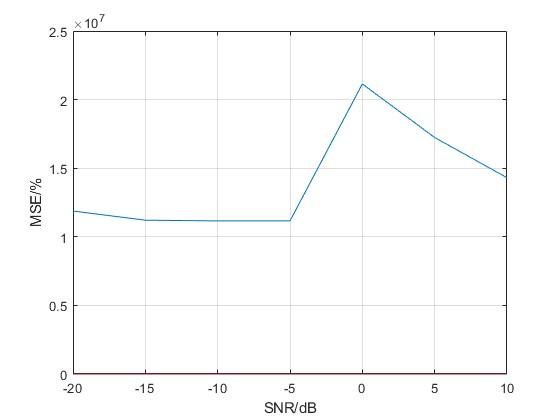
\includegraphics[width=0.8\linewidth]{images/2_Application/music.jpg}
\captionof{figure}{MUSIC分解算法频率估计结果} 
\justifying

这张图展示了使用MUSIC算法进行频率估计时,均方误差(MSE)随信噪比(SNR)变化的情况。MUSIC算法是一种基于子空间方法的频率估计算法,通常用于处理有多个信号源的情况,并且在高信噪比下表现出较好的性能。

从图中可以看到,当SNR从-20dB逐渐增加到10dB时,MSE的变化趋势较为复杂。在SNR从-20dB增加到-5dB的过程中,MSE逐渐降低,这表明在信噪比提高的过程中,MUSIC算法能够更准确地估计出信号的频率。然而,当SNR接近0dB时,MSE急剧上升,达到一个峰值,随后又随着SNR的进一步增加而下降。

这种在中等SNR值附近出现的峰值可能是由于MUSIC算法在处理特定信噪比水平的信号时,由于内部的模型假设或计算限制,导致估计误差突增。这表明MUSIC算法在这个SNR水平可能需要适当的参数调整或模型改进,以提高其在所有信噪比范围内的鲁棒性和精确度。

总的来说,MUSIC算法在大部分信噪比区间内能够较好地工作,但在SNR为0dB左右时表现出一些不稳定性,可能需要进一步的分析和优化以解决这一问题。

\subsubsection{ESPRIT算法实现频率估计}
ESPRIT(Estimation of Signal Parameters via Rotational Invariance Techniques)算法是一种用于估计信号参数的高精度方法,特别适用于超分辨率频率估计和方向估计。该算法利用了信号子空间的结构和旋转不变性原理,通过将信号子空间投影到子空间旋转不变的方向上,实现了对信号频率的准确估计。\cite{roy1989esprit}

下面是ESPRIT算法的基本步骤:

\begin{itemize}
    \item \textbf{构建数据矩阵:} 将接收到的信号数据转换为数据矩阵形式,其中每一列表示一个接收到的信号样本。
    
    \item \textbf{计算信号子空间:} 对数据矩阵进行奇异值分解(SVD),得到信号子空间的估计。
    
    \item \textbf{构建共轭子空间:} 利用信号子空间的性质,构建与之正交的共轭子空间。
    
    \item \textbf{计算估计矩阵:} 通过共轭子空间的特征向量,构建估计矩阵。
    
    \item \textbf{提取信号频率:} 对估计矩阵进行特征分解,得到信号频率的估计值。
\end{itemize}


根据上述描述,可以得到以下思路:


\begin{itemize}
    \item \textbf{构建数据矩阵:} 将接收到的信号数据按时间序列转换为数据矩阵形式,其中每一列代表一个信号样本。这里的变量为 \texttt{signal},表示信号矩阵;\texttt{fs} 表示信号的采样率。
    
    \item \textbf{SVD分解:} 对数据矩阵进行奇异值分解(SVD),得到信号子空间的估计。在这里,使用了MATLAB内置函数 \texttt{svd} 进行奇异值分解。
    
    \item \textbf{选择信号子空间:} 从SVD结果中选择信号子空间。这里的变量为 \texttt{U},表示SVD分解后的左奇异向量矩阵。
    
    \item \textbf{解相位:} 对所选信号子空间中的特征向量进行相位解析,得到频率的相位。这里的变量为 \texttt{phi},表示相位。
    
    \item \textbf{转换为频率:} 将相位转换为对应的频率值。这里的变量为 \texttt{fc},表示估计出的频率。
    
    \item \textbf{确保频率为正值:} 最后,确保所有估计出的频率都是正值。
\end{itemize}

\begin{lstlisting}
function fc = esprit_function(signal, fs)
    % ESPRIT算法的MATLAB实现
    %   signal: 信号矩阵,每一列代表一个信号
    %   fs: 信号采样率
    %   输出fc为ESPRIT算法估计出的频率

    % 假定信号是已经通过FFT处理过的
    n = size(signal, 1); % 信号长度
    d = size(signal, 2); % 信号数量

    % 初始化频率数组
    fc = zeros(d, 1);

    % 对每个信号执行ESPRIT算法
    for k = 1:d
        % 构造数据矩阵
        X1 = signal(1:end-1, k);
        X2 = signal(2:end, k);

        % SVD分解
        [U, ~, ~] = svd([X1, X2], 'econ');

        % 选择信号子空间
        Us = U(:,1);

        % 解相位
        phi = angle(Us(end) / Us(1));

        % 转换为频率
        fc(k) = fs * phi / (2 * pi);
    end

    % 确保所有频率为正值
    fc = abs(fc);
end

\end{lstlisting}

可以得到以下结果:

\centering 
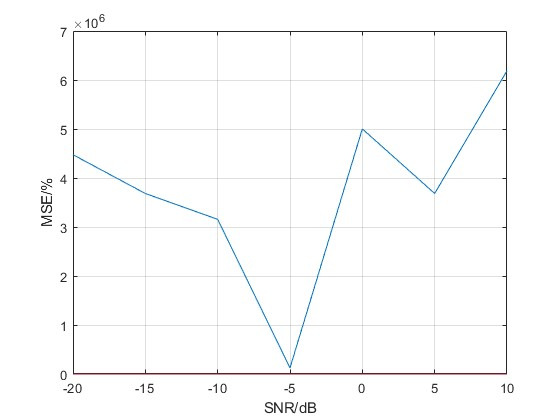
\includegraphics[width=0.8\linewidth]{images/2_Application/esprit.jpg}
\captionof{figure}{ESPRIT算法频率估计结果} 
\justifying

这张图显示了使用ESPRIT算法进行频率估计时,均方误差(MSE)随信噪比(SNR)变化的趋势。ESPRIT算法是一种流行的参数估计技术,它利用信号的子空间特性来估计信号参数,特别是在存在多个信号源时表现出较高的精度。

从图中可以看出,当SNR从-20dB增加到-5dB时,MSE逐渐降低,并在-5dB时达到最小值,这表明在这个信噪比水平下,ESPRIT算法能够非常准确地估计出信号的频率。这可能是因为在-5dB的信噪比下,ESPRIT算法成功地区分了信号子空间和噪声子空间,从而获得了较高的估计准确性。

然而,当SNR继续增加至0dB和5dB时,MSE开始上升,这可能是由于算法在处理较高信噪比下的信号时,面临新的挑战,比如模型过拟合或信号处理中的其他复杂因素。在10dB的信噪比下,MSE再次显著增加,这可能是因为在极高的信噪比环境下,算法的某些假设不再适用,导致估计性能下降。

这个结果表明,尽管ESPRIT算法在中等信噪比水平(如-5dB)下表现优异,但在更高或更低的信噪比下可能需要进一步的调整或优化。这可能包括调整算法的内部参数,改进信号模型,或者采用更复杂的信号处理技术来改善其在各种环境下的性能。


\subsubsection{Capon谐波分解算法实现频率估计}
Capon谐波分解算法是一种频谱估计方法\cite{capon1969high},用于在噪声干扰下准确地估计信号的频率。该算法基于最小方差准则,通过优化空间谱估计来提高频率估计的精度。以下是该算法的主要步骤:


\begin{itemize}
    \item \textbf{构建数据矩阵:} 将接收到的信号数据按时间序列转换为数据矩阵形式,其中每一列代表一个接收到的信号样本.
    \item \textbf{计算协方差矩阵:} 对数据矩阵进行协方差矩阵的计算,该矩阵反映了信号的统计特性.
    \item \textbf{空间谱估计:} 基于协方差矩阵,利用空间谱估计方法计算信号的谱密度函数,即空间谱.
    \item \textbf{最小方差准则:} Capon谐波分解算法采用最小方差准则来优化空间谱估计,以提高频率估计的精度。通过最小化噪声方差,得到更准确的信号频率估计值.
    \item \textbf{频率估计:} 通过分析优化后的空间谱,识别出峰值对应的频率作为信号的频率估计值.
\end{itemize}


Capon谐波分解算法的优点在于对信号和噪声的空间结构进行了充分利用,能够在噪声干扰较大的情况下实现准确的频率估计。

根据上述描述,可以得到以下思路:

\begin{itemize}
    \item \textbf{获取信号大小信息:} 通过 \texttt{size()} 函数获取信号矩阵的大小信息,以确定信号的长度和数量。
    
    \item \textbf{初始化输出频率数组:} 根据信号数量初始化一个数组,用于存储估计得到的频率值。
    
    \item \textbf{对每个信号进行处理:} 使用循环逐个处理每个信号。
    
    \item \textbf{获取单列频谱数据:} 从频谱矩阵中提取出当前信号的频谱数据。
    
    \item \textbf{计算自相关:} 对频谱数据进行傅里叶逆变换,并取其模的平方,得到自相关值。
    
    \item \textbf{生成自相关矩阵:} 根据自相关值构建自相关矩阵。
    
    \item \textbf{确保自相关矩阵是正定的:} 为了避免矩阵不正定导致计算问题,对自相关矩阵进行微小的修正。
    
    \item \textbf{Capon谱估计:} 根据Capon谐波分解算法的原理,计算每个频率点上的Capon谱估计值。
    
    \item \textbf{找到谱峰:} 在Capon谱估计结果中找到最大值对应的位置,即为估计的频率。
    
    \item \textbf{计算估计的频率:} 将谱峰的位置转换为对应的频率值,并存储在输出频率数组中。
\end{itemize}

\begin{lstlisting}
function fc = capon_function(spec, fs)
    % Capon谐波分解算法的MATLAB实现
    %   spec: 信号频谱列向量或以列向量叠加的矩阵
    %   fs: 信号采样率
    %   输出fc为Capon算法估计出的频率

    % 获取信号的大小信息
    [nfft, signalNum] = size(spec);
    fc = zeros(1, signalNum); % 初始化输出频率数组
    
    % 对每个信号进行处理
    for k = 1:signalNum
        % 获取单列频谱数据
        spectrum = spec(:, k);

        % 计算自相关
        autocorr_values = ifft(abs(spectrum).^2);

        % 生成自相关矩阵
        R = toeplitz(autocorr_values(1:nfft/2+1));

        % 确保自相关矩阵是正定的
        R = R + 1e-6 * eye(size(R));

        % Capon谱估计
        capon_spectrum = zeros(nfft, 1);
        for f_idx = 1:nfft
            a = exp(-1j * 2 * pi * (0:(nfft/2)) * (f_idx - 1) / nfft).';
            capon_spectrum(f_idx) = 1 / (a' * inv(R) * a);
        end
        
        % 找到谱峰
        [valueMax, posMax] = max(capon_spectrum);
        
        % 计算估计的频率
        fc(k) = (posMax-1) * fs / nfft;
    end
end

\end{lstlisting}

可以得到以下实验结果:

\centering 
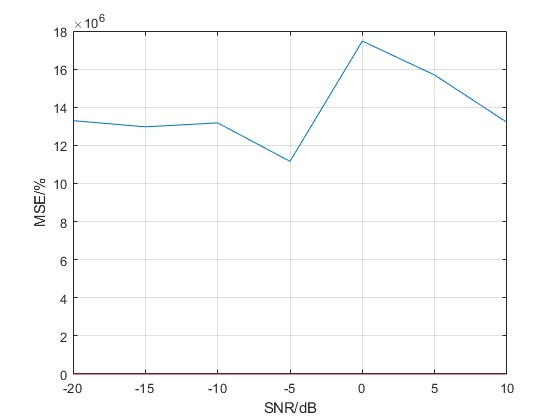
\includegraphics[width=0.8\linewidth]{images/2_Application/capon.jpg}
\captionof{figure}{Capon谐波分解算法频率估计结果} 
\justifying

这张图展示了使用Capon算法(也称为最小方差无失真响应MVDR算法)进行频率估计时,均方误差(MSE)随信噪比(SNR)的变化情况。Capon算法是一种自适应波束形成算法,通常用于提高信号的方向性和抑制噪声。

从图中可以看到,当SNR从-20dB逐渐增加到-5dB时,MSE逐渐降低,并在-5dB处达到最低点。这表明在-5dB的信噪比水平下,Capon算法能够有效地利用信号的统计特性,最大限度地减少估计误差,从而实现较为准确的频率估计。

然而,当SNR从-5dB增加到0dB时,MSE呈现出一个上升趋势,尤其在0dB附近达到一个明显的峰值。这可能是由于算法在这个信噪比区间内的某些特性导致性能下降,例如在处理接近平衡信噪比时可能的参数不稳定或模型的不适应性。随后,当SNR继续增加到10dB时,MSE再次降低。

这种在不同信噪比水平下的性能变化提示Capon算法在极端信噪比条件下,尤其是在信噪比非常接近0dB时,可能需要额外的优化或参数调整来保证其鲁棒性和准确性。在实际应用中,选择合适的模型参数和对算法进行适当的调整将是关键,以确保在各种信噪比环境下都能获得稳定且可靠的频率估计结果。

\subsubsection{主程序部分}
在主程序部分主要包括了加载S.mat信号数据和生成噪声等操作,之后调用上述方法的函数,主要思路如下:

这段代码实现了信号频率估计算法在不同信噪比(SNR)下的性能评估。具体步骤如下:
\begin{itemize}
    \item \textbf{加载信号数据:} 使用 \texttt{load S} 命令加载信号数据。
    \item \textbf{定义信噪比范围和其他参数:} 定义了不同信噪比(SNR)的取值范围,信号的长度(\texttt{N})、采样率(\texttt{fs})和频率(\texttt{f})等参数。
    \item \textbf{生成带有噪声的信号:} 循环迭代了100次,每次循环生成一组带有不同信噪比的信号数据。首先,对原始信号 \texttt{S} 加入不同信噪比的高斯白噪声,得到一组带噪声的信号。然后,对每个信号应用矩形窗口以减小频谱泄漏效应。
    \item \textbf{进行频率估计:} 这部分代码被注释掉了,因为需要根据具体的算法选择合适的函数进行频率估计。你需要用适当的算法函数(如前面介绍的MUSIC、ESPRIT、Capon等)来替换 \texttt{fc=相应算法函数(fft\_signal,fs);} 这行代码。
    \item \textbf{计算估计误差:} 计算了100次估计的频率与真实频率之间的误差。
    \item \textbf{计算均方误差(MSE):} 对每个信噪比下的估计误差进行均方误差的计算。
    \item \textbf{绘制性能曲线:} 将不同信噪比下的均方误差(MSE)绘制成曲线,用于评估不同信噪比下频率估计算法的性能。
\end{itemize}



这段代码用于评估信号频率估计算法在不同信噪比下的性能表现,但实际使用时需要替换其中的 \texttt{replace\_the\_function\_above} 部分为具体的频率估计算法函数,并根据需要调整其他参数。

\begin{lstlisting}
clc;clear;close all;

load S;
SNR=[-20,-15,-10,-5,0,5,10];
SNR_n=length(SNR);
N=78;
n=1:N;
fs=8000;
f=352;
signal = zeros(N,SNR_n);

err=zeros(100,SNR_n);
for i=1:100
    for k = 1:SNR_n-1
        signal(:,k+1) = awgn(S,SNR(k));
    end
    signal(:,1) = S;

    rect = rectwin(N);
    signalRectWin = repmat(rect,1,SNR_n).*signal; 
    fft_signal=real(fftshift(fft(signalRectWin)));
    fc=replace_the_function_above(fft_signal,fs);
    err(i,:) = fc-f;
end

err_mse=zeros(SNR_n);
for j=1:SNR_n
    err_mse(j)=mse(err(:,j));
end

plot(SNR,abs(err_mse));
grid on;
xlabel('SNR/dB');
ylabel('MSE/%');


\end{lstlisting}
\newpage
\bibliographystyle{unsrt}
\bibliography{bibliography/exp2}


\end{document}